\paragraph{\glspl{workpiece} und Sortierung}
\begin{itemize}
    \item[REQ-1:] Die Anlage kann zwischen vier Typen von \glspl{workpiece}n unterscheiden (2, 3, 4, 5, 6)
    \begin{itemize}
        \item \gls{workpiece_flach} (3)
        \item \gls{workpiece_metall} (4)
        \item \gls{workpiece_bohrung} (5)
        \item \gls{workpiece_hoch} (6)
    \end{itemize}
    \item[REQ-2:] Am Ende des 2.\ Förderbandes sollen die \glspl{workpiece} zyklisch in folgender Reihenfolge ankommen (1,7,8)
    \begin{enumerate}
        \item \gls{workpiece_metall}
        \item \gls{workpiece_bohrung}
        \item \gls{workpiece_flach}
    \end{enumerate}
    \item[REQ-3:] \glspl{workpiece}, die nicht in die Sortierreihenfolge passen werden in eine der beiden Rutschen aussortiert (9, 10)
    \item[REQ-4:] Der \gls{durchsatz} an \glspl{workpiece} ist zu optimieren (11)
    \item[REQ-30:] Aussortierung der \glspl{workpiece} soll mit \gls{weiche} funktionieren (41)
    \item[REQ-38:] Aussortierung der \glspl{workpiece} soll mit \gls{ejector} funktionieren (41)
    \item[REQ-39:] Beliebige Kombinationen der \gls{sortierer} an den beiden \glspl{anlage} sollen unterstützt werden. (42)
    \item[REQ-47:] Wenn ein \gls{workpiece_bohrung} oder \gls{workpiece_metall} umgedreht wird, ist es ein \gls{workpiece_hoch}.
\end{itemize}

\paragraph{Kapazität}
\begin{itemize}
    \item[REQ-5:] Eine volle Rutsche ist an der Anlage zu signalisieren (12)
    \begin{itemize}
        \item "LED ""Rutsche voll"" an der Anlage soll angeschaltet werden."
    \end{itemize}
    \item[REQ-6:] Wenn die nächste notwendige Aussortierung aufgrund von ausgeschöpfter Rutschenkapazität
    nicht stattfinden kann, wird der Gesamtbetrieb gestoppt (13)
\end{itemize}

\paragraph{Durchlassablauf}
\begin{itemize}
    \item[REQ-7:] Zuführung von Werkstücken erfolgt durch Einlegen von Werkstücken in der
    Lichtschranke am Anfang von Förderband 1 (14,15)
    \begin{itemize}
        \item Ein Unterbrechen der Lichtschranke signalisiert dem System das Einlegen eines Werkstücks,
        sodass mit dem Sortiervorgang von diesem begonnen werden kann.
    \end{itemize}
    \item[REQ-9:] Das System muss mit in beliebigem Abstand eingelegten Werkstücken umgehen können(16,17)
    \begin{itemize}
        \item Solange der Bereich der ersten Lichtschranke frei ist, muss der Benutzer Werkstücke
        einlegen können, ohne die Korrektheit der Funktion zu gefährden.
    \end{itemize}
    \item[REQ-14:] Der Abstand von Werkstücken auf Förderband 2 muss mindestens 25 cm betragen (18)
    \begin{itemize}
        \item Bedingung muss vor der Übergabe sichergestellt werden
    \end{itemize}
    \item[REQ-16:] Auf dem Förderband von Anlage 2 dürfen sich maximal 2 Werkstücke befinden (19)
    \begin{itemize}
        \item Muss bei der Übergabe sichergestellt werden
    \end{itemize}
    \item[REQ-18:] Falls sich bei der Übergabe zwischen den beiden Förderbändern ein Werkstücke
    überschlägt, muss der neue Werkstücktyp beachtet werden. (20)
    \begin{itemize}
        \item Wir schließen den Fall aus, dass das Teil auf die Seite fällt, sodass es wegrollen könnte.
        Wenn sich das Werkstück überschlägt, ändert sich bei hohen Werkstücken der Typ.
    \end{itemize}
    \item[REQ-20:] Werkstücke dürfen nicht vom Band fallen (21)
    \item[REQ-24:] Beim Einlegen eines Werkstückes in die Anlage soll diesem eine eindeutige ID zugewiesen werden(28)
    \item[REQ-26:] Wenn sich auf einem Förderband kein Werkstück befindet, stoppt dieses.
    \item[REQ-31:] Wenn ein Werkstück die Lichtschranke am Ende von FB2 erreicht,
    sollen Informationen dazu auf der Konsole ausgegeben werden (22, 23, 24, 25, 26, 27)
    \begin{itemize}
        \item Zu den Informationen zählen die ID, Typ, Höhe auf FB1 und FB2 des Werkstücks als
        auch ein Hinweis darüber, ob sich das Werkstück überschlagen hat.
    \end{itemize}
\end{itemize}

\paragraph{Bedienung durch Taster}
\begin{itemize}
    \item[REQ-12:] Bei Betätigung des START-Tasters wechselt die Anlage in den Betriebszustand (49)
    \item[REQ-15:] Bei Langem Drücken von drei Sekunden des START-Tasters wechselt die Anlage in den Service-Modus (50)
    \begin{itemize}
        \item Im Service Modus führt die Anlage Kalibrierung und Selbsttests durch.
        Anforderung hierfür ist, dass die Anlage im Ruhezustand ist.
    \end{itemize}
    \item[REQ-17:] Bei Betätigung des STOPP-Tasters wechselt die Anlage in den Ruhezustand (51, 52)
    \begin{itemize}
        \item Dafür müssen bestehende Fehler behoben und quittiert und gegangene Fehler quittiert sein.
        Alles andere führt zu einer Fehlermeldung.
    \end{itemize}
    \item[REQ-21:] Bei Betätigung des RESET-Tasters werden sämtliche Fehler quittiert (53)
    \item[REQ-28:] Wenn die Anlage durch ESTOPP stillgelegt ist, kann der Betrieb durch Drücken des
    RESET-TASTERs der Anlage, an dem auch der E-Stopp-Schalter gedrückt wurde, fortgesetzt werden (56)
    \begin{itemize}
        \item Bedingung dafür: Keine ESTOPP-Schalter sind gedrückt
    \end{itemize}
    \item[REQ-40:] Im Service Modus führt die Anlage beispielsweise Kalibrierung und Selbsttests durch (50)
    \begin{itemize}
        \item Aus dem Anforderungsdokument geht dies nicht eindeutig hervor, dies muss in zukünftig spezifiziert werden.
    \end{itemize}
    \item[REQ-41:] Bei Betätigung des ESTOPP-Schalters werden beide Förderbandmodule angehalten (54, 55)
    \item[REQ-42:] Dem Benutzer werden Hinweise über die Benutzung der Anlage mithilfe der LEDs an der Tastatern gegeben
    \begin{itemize}
        \item Im Betriebszustand ist die LED am Start-Taster an, im Ruhezustand die LED am Stopptaster.
        Bei einem gegangenen oder bestehenden Fehler ist die LED am RESET-Taster an.
    \end{itemize}
\end{itemize}

\paragraph{Zustandsanzeigen}
\begin{itemize}
    \item[REQ-10:] Im Betriebszustand leuchtet die Lampe grün dauerhaft (59)
    \item[REQ-11:] Im Service-Mode blinkt die Lampe grün (60)
    \item[REQ-13:] Bei Warnungen blinkt die Lampe gelb (61)
    \begin{itemize}
        \item Eine Warnung ist, dass die Rutsche an der Anlage voll ist.
    \end{itemize}
    \item[REQ-19:] Wenn keine Warnungen vorliegen ist die gelbe Lampe aus (61)
    \item[REQ-37:] Die rote LED signalisiert die Fehlerzustände wie folgt (73, 74, 75, 76):
    \begin{itemize}
        \item Anstehend unquittiert wird durch schnelles Blinken (1 Hz) signalisiert (74).
        Anstehend quittiert wird durch dauerhaftes Leuchten(75) signalisiert.
        Gegangen unquittiert wird durch langsames Blinken (0,5 Hz) signalisiert (z.B.\ wenn ein
        Werkstück an einer Weiche zu langsam in die Rutsche geschoben wurde) (76).
        Steht kein Fehler an, ist die Leuchte aus (73).
    \end{itemize}
    \item[REQ-45:] Im Ruhezustand leuchtet die Lampe dauerhaft gelb
\end{itemize}

\paragraph{Weiche}
\begin{itemize}
    \item[REQ-23:] Verklemmen der Weiche soll überwacht werden (37)
    \begin{itemize}
        \item Ein Werkstück ist verklemmt, wenn das Werkstück, abzüglich der Toleranz von 50 Prozent
        der durchschnittlichen Aussortierzeit, länger als erwartet braucht, um in der Rutsche anzukommen.
        Daraufhin wird eine Warnung ausgesendet, bis das Teil in der Rampe ankommt.
    \end{itemize}
    \item[REQ-27:] Die Weiche darf nicht länger als 'x' auf offen stehen (35, 36)
    \begin{itemize}
        \item Bei minutenlangen Stromfluss wird die Weiche beschädigt.
    \end{itemize}
\end{itemize}

\paragraph{Embedded Recorder}
\begin{itemize}
    \item[REQ-25:] Es soll eine 'record'-Funktion bereitgestellt werden, mit der ein Benutzer das gesamte
    Ereignisprotokoll der Anlage aufzeichnen kann (90)
    \item[REQ-29:] Die von der 'record'-Funktion vorgenommene Aufzeichnung soll menschenlesbar sein (91)
    \item[REQ-33:] Es soll eine 'replay'-Funktion bereitgestellt werden, mit der ein
    Benutzer eine zuvor aufgezeichnete Ereignissequenz abspielen lassen kann (93, 94)
    \item[REQ-34:] Ereignissequenzen sollen per Hand angefertigt werden können (95, 96)
\end{itemize}

\paragraph{Höhenmessung}
\begin{itemize}
    \item[REQ-32:] Höhenmessung muss Kippung des Lasers mit einbeziehen (43, 44)
\end{itemize}

\paragraph{Fehlerumgang}
\begin{itemize}
    \item[REQ-35:] Nach Behebung eines Fehlers soll der Normalbetrieb fortgesetzt werden. (45, 46)
    \begin{itemize}
        \item Nach Möglichkeit sollen die Laufbänder nicht geräumt werden.
    \end{itemize}
    \item[REQ-43:] In den Zuständen 'bestehend\_unquittiert' und 'bestehend\_quittiert' bleiben die
    Laufbänder beider Anlagen stehen und den Aussortiermechanismen wird der Strom abgestellt
    \begin{itemize}
        \item Die Fehleranzeige über die Ampel ist in REQ-37: spezifiziert
    \end{itemize}
    \item[REQ-36:] Fehlerzustand soll wie in Abbildung~\ref{fig:stm-fehlerzustand} beschrieben sein. (65, 66, 67, 69, 70)
    \item[REQ-46:] Der globale Fehlerzustand wird wie folgt festgelegt
    \begin{itemize}
        \item Der aktuell bestehende Fehler mit der höchsten Priorität entspricht dem Fehlerzustand der gesamten Anlage.
        Die Fehlerzustände sind der folgenden Liste nach priorisiert: 1.\ Anstehend unquittiert
        2.\ Anstehend quittiert 3\ Gegangen unquittiert 4.\ OK
    \end{itemize}
\end{itemize}

\begin{figure}[h]
    \centering
    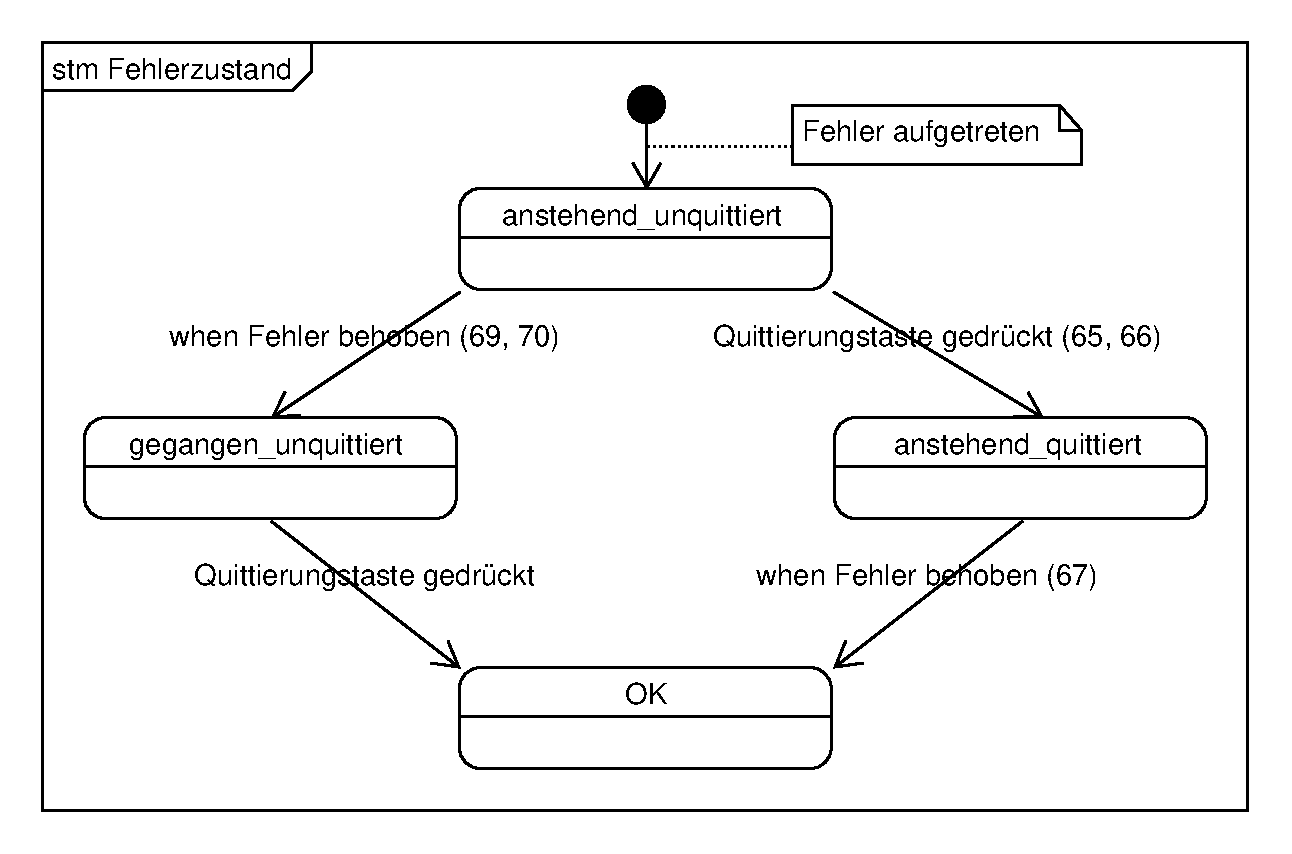
\includegraphics[scale=0.5]{../out/diagrams/stage1/req-fehlerzustand}
    \caption{REQ-36 Visualisierung des Fehlerzustandes eines einzelnen Fehlers}
    \label{fig:stm-fehlerzustand}
\end{figure}
